\documentclass[draft,english]{jflart}
\usepackage[utf8]{inputenc}
\usepackage[T1]{fontenc}
\usepackage{lstcoq}
\usepackage[numbers]{natbib}
\usepackage{enumitem}
\usepackage{subcaption}

% Numéro et année des JFLAs visées par l'article, obligatoire.
\jfla{36}{2025}

%\title{Functorial Symmetric Cryptography}
\title{Can Symmetric Cryptography Be Liberated from the Von Neumann
  Style?}
\titlerunning{Free Von Neumann!}

% Auteurs
\author[1]{Jean-Baptiste Menant}
\author[2]{Yves Ndiaye}
\author[2,3]{\\Pierre-Évariste Dagand}
\authorrunning{Menant, Ndiaye et Dagand}

% Affiliations des auteurs
\affil[1]{École Normale Supérieure de Lyon}
\affil[2]{Université Paris Cité, IRIF}
\affil[3]{CNRS}

\newcommand{\TODO}[1]{\textcolor{red}{$\langle$ TODO:}#1\textcolor{red}{$\rangle$}}
\newcommand{\ie}{\textit{i.e.}}
\newcommand{\etc}{\textit{etc.}}

\newcommand{\Skinny}{\textsc{Skinny}}
\newcommand{\Gift}{\textsc{Gift}}
\newcommand{\AES}{\textsc{Aes}}
\newcommand{\DES}{\textsc{Des}}

\begin{document}

\maketitle

\begin{abstract}

  In defiance of Hinchliffe's rule, this article sets out to
  demonstrate that its title can be answered by the word ``yes''. We
  show that modern symmetric ciphers can be modeled through a small
  set of algebraic structures (Boolean algebra, Naperian and circulant
  functors). We reveal that these ciphers exhibit some interesting
  compositional structure at the type-level. This enables systematic
  code transformation, known in the cryptographic folklore as
  ``bitslicing'' and ``fixslicing''. Our work rests on a Coq
  development providing the specification of two ciphers, \Skinny{} and
  \Gift{}, deriving a bitsliced and fixsliced implementation for each and
  proving their correctness with respect to their specifications.

\end{abstract}

\section{Introduction}

%% * Amazing cryptographers (ZRR)
%% "trade secret"
%% "genius out of the bottle", like toothpaste
%% ** Section 2: F_{}
%% ** Section 5: Cortex ARM M4 assembly
%% -> Our offer: Section 4
%%   -> shorter Section 5

Anyone who has ever read a cryptography paper knows this for a fact:
cryptographers are at the top of the academic thought chain. In the
archetypal symmetric cryptography paper, there is a ``Section 2''
scene in which cryptographers are bravely waving their most potent
finite field. In a latter ``Section 4'' scene, the very same
cryptographers are seen extolling the virtues of some nifty
\textsc{Arm} Cortex assembly instruction, which takes center stage in
their hand-crafted, manually optimized implementation. No wonder we
jealously stash them away in ``zone à régime restrictive''! The rumor
goes that, behind these padlocked doors, they have developed a set of
domain-specific techniques to deliver high-throughput software
implementation of symmetric ciphers. This has been slowly gnawing at
compiler writers, whose job security is now
threatened~\citep{bernstein:death-compiler,venkatesh:compiler-security}.
Luckily for us, every now and then, someone inadvertently let the
genies out of their Klein bottle and we get to read about the subtle
art of ``bitslicing''~\citep{biham:DES} and
``fixslicing''~\citep{adominicai:fixslicing-gift,
  adomnicai:fixslicing-AES-like}.

The present work aims at casting these two notions in the language of
functional programming. We shall see that bitslicing corresponds to a
run-off-the-mill \emph{data} representation change (in effect, a
matrix transposition). But this is only half of the work: our ability
to systematically transform the \emph{code} operating on such
representation rests on suitably polymorphic definitions:
parametricity at its best! Fixslicing, on the other hand, will be
rationalized through equational reasoning over purely functional
terms. Identifying commuting expressions is of key importance there:
programming with algebraic structures (rather than untamed arrays of
bits) will be instrumental!

In the long run, our ambition is to offer cryptographers the
conceptual apparatus to better illuminate their ``Section 4'' scene.
Each and every symmetric cryptosystem should not have to exhibit a
bitsliced or fixsliced implementation: by just \emph{specifying} the
cryptosystem in the right framework (abstract yet suitably
operational), one should get the guarantee that the design can be
bitsliced and fixsliced. In fact, one would boldly claim that a
compiler could automatically apply these transformations and produce
optimized code, starting from an high-level description of the cipher.
This is already the case for bitslicing~\citep{mercadier:PhD}, adding support
for fixslicing is next on the list.

%% * Executive summary of modern symmetric cryptography
%% ** iterate pure `round` function N times
%% *** thread a `state`
%% **** initially: clear text
%% **** finally: cipher text
%% *** mixing in constants derived from a secret key
%% **** computed off-line
%% **** off the critical path

As intimidating as cryptographers are, the essence of modern symmetric
cryptographic primitives can in fact be distilled in a few paragraph. A
primitive can be understood as a purely functional program. It takes
two inputs: the ``cleartext'' and a list of ``round subkeys''
(which are derived from a single key through a non-performance-critical process called ``key schedule'' that we shall ignore here).
The output is the ``ciphertext''. The cleartext, the ciphertext and
each individual round subkeys are processed as ``blocks'' of binary
data. The block size is of the order of a hundred bits (typically, 64, 128
or 256 bits).

Looking at the process of turning the cleartext into a ciphertext, one
realizes that cryptographers have been programming in the State monad
all along: ciphers are described as operating on a ``state'',
initialized to be the cleartext and read off at the end as the
ciphertext. This state is updated by a ``round'' function that is
repeated a given number of times (of the order of ten iterations). The
exact number of iterations is a trade-off between latency (less
iterations means faster computation) and security (more iterations
makes for more costly cryptanalysis effort). The round function itself
is built compositionally from 3 components: a key mixing layer (making
the encryption process reversible), a confusion layer (smoothing local
correlations among the inputs) and a diffusion layer (spreading
correlations across the whole output block).

%% ** side-channel attack
%% *** no control-flow
%% **** only statically bounded loops
%% *** no memory access based on data flow
%% **** only register spilling
%% *** -> combinational circuits

To avoid side-channel attack (for example, based on
timing~\citep{bernstein:timing-attack-AES}) over software
implementations, this pipeline is implemented as a purely
combinational circuit. In particular, we are forbidden from performing
control-flow operations on secret data, leaving only
statically-bounded loops. We are also forbidden from performing memory
access based on the secret data, leaving only register spilling.

%% ** modernity: starts with AES
%% *** more structured than DES
%% *** in particular: no-trick-up-my-sleeves Sbox
%% ** operate over bit-level n-dimensional array

Following the NSA involvement in the design of the \DES{} confusion
layer~\citep{johnson:cold-war-crypto}, cryptographers have been
advocating for ``nothing-up-my-sleeve'' designs (which does not make
magic tricks impossible, just
harder~\citep{bernstein:something-up-my-sleeves}). For example, the
confusion layer of the \AES{} standard is based on the usual
multiplicative inverse over the finite field induced by an
innocent-looking polynomial. To support such designs, the state modern
ciphers operate on is taken to represent a certain matrix
(oftentimes, a 2D or 3D array of bits): the cipher is not specified
over a flat sequence of individual bits but over a n-dimensional array
of bits.

%% ** designed for high-throughput execution in software 
%% *** -> parallel execution
%% *** -> "scale out" on SIMD

Moreover, ciphers are now, by and large, designed to be run
efficiently on software. The era of hardware-based cryptography is
long gone, even for embedded
platforms~\citep{buchanan:nist-lightweight-crypto}. To achieve
high-throughput, ciphers are typically designed so as to admit a
bitsliced implementation. Bitslicing enables a form of parallel
execution \emph{within} machine words, relying sometimes explicitly on
the availability of vectorized instructions~\citep{beaulieu:speck,
  bernstein:chacha}. We thus gain access to a form of CPU-level
``scale out'' to larger machine words, in particular through
single-instruction multiple-data (SIMD) instructions. Doubling the
size of machine words yields nearly twice the throughput, without any
effort. Evidence tends to suggest that cryptographers obtain bitsliced
designs through sheer intellectual might. It is in fact the sole
purpose of the traditional ``Section 4'' scene to exhibit a bitsliced
witness in all the gory details.

%% * Contributions
%% ** identify algebraic structure
%% *** mathematical language of software circuits
%% ** rationalize bitslicing
%% *** representation change
%% *** -> key ingredient: parametricity
%% ** rationalize fixslicing
%% *** split & commute permutations
%% *** -> key ingredient: equational reasoning

What would it take to turn this art form into an engineering
principle? To answer, we make the following contributions:
%
\begin{itemize}
\item we identify the algebraic structure necessary to model modern
  symmetric cryptographic primitives and, in particular, their state
  (Section~\ref{sec:spec}). Doing so, we delineate a mathematical
  language of software circuits, rooted in the categorical notion of
  functor to account for data containers~;
\item we give a formal account of bitslicing as a data representation
  change supported by suitably polymorphic definitions
  (Section~\ref{sec:bitslicing}). As expected when it comes to
  switching between data representations, parametricity plays a key
  role to justify the equivalence of the resulting programs~;
\item we give a formal account of fixslicing as a whole-program
  transformation (Section~\ref{sec:fixslicing}). We show how a
  fixsliced implementation can be obtained through equational
  reasoning. To support such reasoning, we crucially rely on the
  algebraic structure set forth in Section~\ref{sec:spec}.
\end{itemize}

%% ** broader take-away: "functor-oriented programming"
%% *** abstracting over concrete data containers
%% *** modeled as functor + structure (Gibbons)
%% **** -> algebraic reasoning / optimization
%% **** -> turn code back to polymorphic = free theorems
%% ** terminology: "functor" means "categorical functor"
%% *** formally defined in due time

We believe that there is also a broader take-away for an audience of
French functional programmers. The present work surfs on
the wake of the Squiggol school of programming~\citep{bird:squiggol}.
Because our government-approved programming language does not yet
support ad-hoc polymorphism~\citep{white:modular-implicit}, the French
community may be missing out on some interesting programming patterns.
The present article can thus be read as a case-study in
``functor-oriented programming''~\citep{roconnor:functor-oriented},
where the notion of functor comes from category theory (recalled in
Section~\ref{sec:spec} and unrelated to the notion used in ML module
systems). In effect, we forbid ourselves from programming over a
concrete data structure: instead, we rely on (categorical) functors,
peppered with some more structure, so as to 1. unlock algebraic
manipulation during compilation and 2. fully exploit parametricity for
reasoning.

%% * Purely semantics work
%% ** hence: "maybe"
%% ** /> Coq
%% *** -> executability
%% **** -> testing
%% *** -> prototype compiler
%% **** -> `autorewrite`
%% *** some level of confidence
%% *** past experience with Usuba

The present work is but the beginning of our research program. We
shall focus \emph{exclusively} on the semantics aspects, only briefly
touching upon implementation aspects (which remain the raison d'être
of the project!). Our experience designing the Usuba~\citep{mercadier:PhD}
programming language and implementing its compiler gives us some
confidence that a syntax can indeed be tailored to dress up this
semantics.

We nonetheless could not resist the temptation of developing the
semantics in the Coq theorem prover, as executable programs. After
all, we are interested in combinational circuits: if there has ever
been a time where we do not have to worry about termination, this is
it! So we have implemented cryptographic primitive in pure Gallina,
following the lead of some of our colleagues who went even further,
down to deeply-embedded assembly code~\citep{chlipala:coq-crypto}.
Besides the ability to prove the correctness and, even more usefully,
test our code, this also enables us to easily prototype a fixslicing
compiler, using Coq's \texttt{autorewrite} tactics to emulate a
transformation-based simplification
engine~\citep{peyton-jones:haskell-optim} (as part of a fictional
optimizing compiler).


%% * Internship work
%% <- JB: BSc on Skinny
%% <- Ndiaye: MSc on Gift
%% -> running examples: Skinny

%% * Disclaimer: none of these "programs" were easy to write / theorems easy to assert
%%   <- don't be fooled by the magician's trick
%%   -> all the more reason to write a language!
%%     -> automatically inhabit the semantics
%%   -> all the more reason to write a compiler!
%%     -> automatically apply theorems

This article grew out of the Bachelor's research project of the first
author and the Master thesis of the second author. The former worked
on the specification, bitslicing and fixslicing of the \Skinny{}
cipher~\citep{beierle:skinny, adomnicai:fixslicing-AES-like}. The
latter worked on the specification, bitslicing and fixslicing of the
\Gift{} cipher~\citep{subhadeep:gift, adominicai:fixslicing-gift}. Both
ciphers are provided in the accompanying source
code\footnote{\url{https://github.com/pedagand/bitfix}}. For clarity,
we shall focus exclusively on \Skinny{} as our running example here.

Note that none of the programs below were easy to write in the first
place: it took weeks of careful study to weed out the essential
complexity from the accidental mismanagement of array indices. If the
code seem somewhat trivial, one should bear in mind that this
simplicity was hard-won. All the more reason to, some other day,
design a programming language, so as to automatically inhabit this
semantics, and write its compiler, so as to automatically optimize
code following our theorems.

\section{Functional specification}
\label{sec:spec}

%% * Moving beyond "Section 2"
%% ** Operational description
%% ** Non-optimized reference implementation

In this section, we intend to give a specification for the \Skinny{}
cipher, with an eye towards implementation. We shall therefore aim for
a rather operational description, to give a sense of the computational
cost of the cipher, without premature concern for implementation
performance just yet.

%% * Modeling state
%% ** 3 dimensions
%% *** -> figure
%% ** expressed as 3 type formers + (same) structure
%% *** -> introduced incrementally (pedagogy)
%% *** -> summarized in Fig. \ref

As often in functional programming, it helps tremendously to first lay
out the types our program will have to deal with. In our case, the
focal point is the \emph{state} of the cipher, which is specified as a
3-dimensional matrix (Figure~\ref{fig:state}). We model each dimension
in turn through a dedicated type constructor:
%
\begin{itemize}[nosep]
\item \coqe!Rows.T : Type -> Type! is a data container representing 4 rows of data (horizontal dimension),
\item \coqe!Cols.T : Type -> Type! is a data container representing 4 columns of data (vertical dimension), and
\item \coqe!Slice8.T : Type -> Type! is a data container representing
  8 slices of data (depth dimension).
\end{itemize}

The cube drawn in Figure~\ref{fig:state} could just be modeled as
%
\coqe!Rows.T (Cols.T (Slice8.T bool))!,
%
\coqe!Slice8.T (Rows.T (Cols.T bool))!,
%
or any other composition of these 3 type constructors. They are all
isomorphic to a sequence of 128 bits. We shall wait until
Section~\ref{sec:assembling} to settle on the most natural
representation for our specification effort. We revisit this choice in
Section~\ref{sec:bitslicing} when we are concerned with producing a
memory-efficient representation.

\begin{figure}
  \begin{center}
    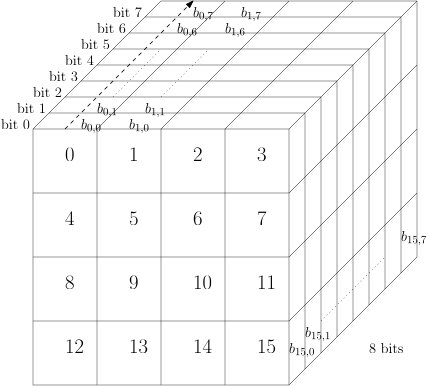
\includegraphics[draft=false,height=5cm]{skinny_state}
  \end{center}
  \caption{\Skinny{} state matrix}
  \label{fig:state}
\end{figure}

%% * Structure: functor
%% ** essence of data container
%% ** contains & preserves collection of individuals
%% ** abstract reading: truely parametric collection (free theorem)


For all intents and purposes, these type constructors shall remain
abstract throughout this article: we interact with them solely through
their algebraic interface. The first of which is the categorical
notion of functor:
%
\coqfrom{Algebra}{Functor}

To the disciples of Reynolds and Girard, this signature has come to
mean ``parametric data container'': how would you go about asserting
that the type constructor \coqe!Rows.T! is not doing something
non-trivial with the type it is provided as an argument? In other
words, how to be sure that a \coqe!Rows.T bool! behaves ``similarly''
as a \coqe!Rows.T nat!? One could try and argue that Coq does not
allow pattern matching on types but it is rather unsavory to involve
the design of the whole programming language into this argument.
%
Instead, we require \coqe!Rows.T! to offer a \coqe!map! operation: this
constructively witnesses the fact that a \coqe!Rows.T A! is
(functionally) related to a \coqe!Rows.T B!, as long as we can
(functionally) relate \coqe!A! and \coqe!B!. Put otherwise, we ask
that \coqe!Rows.T!, and similarly \coqe!Cols.T! and \coqe!Slice8.T!,
come equipped with their free theorems~\citep{reynolds:parametricity,
  wadler:free-theorem}.

%% * Objective: purely functional model
%% ** rule of the game: "no i, no j"

Having modeled the core data types, we now turn to modeling the cipher
as a purely functional program. To stay clear from the temptation of
array mismanagement, we disallow index arithmetic altogether: no
indexing an array-like structure by \coqe!i+1! or, even worse,
\coqe!j-i! in this paper!

\subsection{Key mixing}

%% * Generically over any Boolean algebra
%% ** obvious: `bool`
%% ** useful: `F bool`
%% *** for any commutative applicative functor F

Much like $\lambda$ in functional programming, the exclusive-or
$\oplus$ features prominently in the cryptographic liturgy. In
particular, it is instrumental to mix the derived keys during
ciphertext computation. For genericity, we model this layer as an
operation defined over any Boolean
algebra~\citep{givant:boolean-algebras}:
%
\coqfrom{Skinny/Base}{addroundkey}

%% * Structure
%% ** `bool` is Boolean algebra
%% ** Rows.T, Cols.T and Slice8.T are commutative applicative functors

The type \coqe!bool! is an obvious instance of a Boolean algebra.
However, any commutative applicative~\citep{mcbride:applicative}
functor \coqe!F! applied to a Boolean algebra also yields a Boolean
algebra (dispatching the Boolean operations pointwise to the
underlying elements). For the sake of completeness, we recall that an
applicative functor offers the following operations:
%
\coqfrom{Algebra}{Applicative}


\subsection{Diffusion}

%% * Naperian functor: functional indexing
%% ** definition
%% ** also known as: representable functor

The role of the diffusion layer is to divert individual bits across the
whole structure. Inevitably, this calls for a notion of indexing.
Naperian functors~\citep{hancock:napierian} identify a type \coqe!Ix! of
indices as the logarithm of an exponential type:
%
\coqfrom{Algebra}{Naperian}
%
through the fact that \coqe!lookup! and \coqe!init! form a bijection.
This is also known as a representable functor in categorical
circles~\citep{maclane:working-categorist}.

%% ** example: Rows.T indexed by Rows.Ix
%% ** example: Cols.T indexed by Cols.Ix
%% ** example: Slice8.T indexed by Slice8.Ix

Following our earlier discussion, we ask for \coqe!Rows.T!
(respectively, \coqe!Cols.T!) to be a Naperian functor indexed by a
set of 4 elements. Similarly, \coqe!Slice8.T! must be a Naperian
functor indexed by 8 elements. We define
%
\coqfrom{Rows}{Ix}
%
as the logarithm of \coqe!Rows.T!,
%
\coqfrom{Cols}{Ix}
%
as the logarithm of \coqe!Cols.T!, and
%
\coqfrom{Slice8}{Ix}
%
as the logarithm of \coqe!Slice8.T!.

Note that we have a notion of indexing but no arithmetic: we remain in
line with our objectives. Note also that being Naperian implies being
a commutative applicative functor. As a corollary, we get that any
combination of \coqe!Rows.T!, \coqe!Cols.T! and \coqe!Slice8.t!
applied to \coqe!bool! yields a Boolean algebra, over which we can
therefore write combinational circuits.

%% ** derived operation: Naperian implies commutative applicative
%% ** derived operation: structure of indices

Applying \coqe!init! to the identity function, we generically compute
the container of indices:
%
\coqfrom{Algebra}{indices}

We can witness the fact that \coqe!Rows.T! contains at least as many
elements as \coqe!Cols.T! through the following construction:
%
\coqfrom{Skinny/Base}{indices_C}

Note that, since they actually have the same number of elements, we
could also go the other way around, defining an inhabitant of
\coqe!Cols.T Rows.Ix!. We do not need this construction for \Skinny{}
but it is necessary for \Gift{}, which proceeds by transposition of a
$4 \times 4$ matrix.

%% * Foldable: left-to-right iteration
%% ** induce: left-to-right order
%% ** derived operation: left and right rotation

The first step of the diffusion process consists in applying a right
rotation over each individual column. However, we do not have enough
structure to identify a ``right'' or ``left'' direction over our
containers. To do so, we introduce the (regretfully ad-hoc\footnote{We
were hoping to be able to piggy-back on the notion of
foldable~\citep{yorgey:typeclassopedia} and Naperian functor to
identify directions. Intuitively, \coqe!fold! denotes a unique
left-to-right traversal order. However, we could only turn this into a
rotation if we asked for a decidable equality over the logarithm of
the functor. We are not sure yet whether we want to make such a
commitment.}) notion of circulant functor
%
\coqfrom{Algebra}{Circulant}
%
taking an \coqe!F!-vector to an \coqe!F! $\times$ \coqe!F! circulant
matrix (performing a right-rotation of \coqe!F A! at each step) and
\coqe!F! $\times$ \coqe!F! anticirculant matrix (performing a
left-rotation of \coqe!F A! at each step).

More usefully for our purposes, we can derive generic left and right
rotation operators for any circulant functor \coqe!T!  Naperian over a
type \coqe!Ix!:
%
\coqfrom{Algebra}{ror_rol_sig}


%% The equational theory is unclearas expected for rotations: additive on the
%% indices when going in the same direction (\coqe!ror i (ror j xs)! and
%% \coqe!rol i (rol j xs)!), subtractive when going in opposite direction
%% (\coqe!ror i (rol j xs)! and \coqe!rol i (ror j xs)!).

%\coqfrom{Algebra}{Foldable}
%% Taking the monoid to be \coqe!list A! (under nil and concatenation,
%% \ie{} the free monoid construction), we can read off the
%% directionality we were after.
%% %

%% * Application: shiftows
%% ** figure: rotate each column by the the row index

After suitable generalization, this leads us to the following model
for the \coqe!shiftrows_! operation, depicted in
Figure~\ref{fig:shiftrows}:
%
\coqfrom{Skinny/Base}{shiftrows}
%
which represents the first half of the diffusion layer.
%
%% * Application: mixcolumns
%% ** figure: psi_ >-> ror 1
%
The second half corresponds to a combinational circuit \coqe!psi_!
%
\coqfrom{Skinny/Base}{psi}
%
which exercises the Naperian structure of \coqe!Rows.T! together with
the underlying Boolean algebra. This is followed by a right rotation
of rows. Altogether, this defines the \coqe!mixcolumns_! operation,
depicted in Figure~\ref{fig:mixcolumns}:
%
\coqfrom{Skinny/Base}{mixcolumns}

\begin{figure}[tp]
  \centering
  \begin{subfigure}[t]{0.45\textwidth}
    \centering
    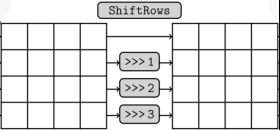
\includegraphics[draft=false,height=2.8cm]{shiftrows}
    \caption{Shiftrows (from~\citet{beierle:skinny})}
    \label{fig:shiftrows}
  \end{subfigure}
  \begin{subfigure}[t]{0.45\textwidth}
    \centering
    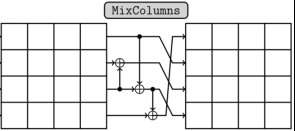
\includegraphics[draft=false,height=2.8cm]{mixcolumns}
    \caption{Mixcolumns (from~\citet{beierle:skinny})}
    \label{fig:mixcolumns}
  \end{subfigure}
  \caption{\Skinny{} diffusion layer}
\end{figure}

\subsection{Confusion}

% * Naperian functor
%% ** derived operation: permutation

The confusion layer builds upon two permutations over \coqe!Slice8.T!.
Once again, this is merely exploiting the Naperian structure of
\coqe!Slice8.T!: for any Naperian functor \coqe!F! indexed by
\coqe!Ix!, there exists a generic permutation operator
%
\coqe!perm : forall A, (Ix -> Ix) -> F A -> F A!.
%
This leads to the following definitions:
%
\coqfrom{Skinny/Base}{perms}

%% * Application: subcells

At the heart of this layer stands the substitution box \coqe!s8!
(Figure~\ref{fig:s8}), which is just another combinational circuit:
%
\coqfrom{Skinny/Base}{s8}

These building blocks are chained together to form the confusion
layer, \coqe!subcells_!:
%
\coqfrom{Skinny/Base}{subcells}

\begin{figure}
  \centering
  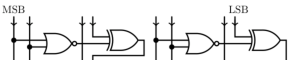
\includegraphics[draft=false,width=.75\textwidth]{s8}
  \caption{Substitution box S8 (from~\citet{beierle:skinny})}
  \label{fig:s8}
\end{figure}

\subsection{Making the rounds}
\label{sec:assembling}

%% * state: natural composition order
%% ** -> thinking required
%% *** /> not necessarily efficient implementation
%% *** -> see sec:bitslicing

A round of \Skinny{} is obtained by composing the following operations in
this particular order:
%
\begin{enumerate}
\item \coqe!subcells_ : forall {B : Type}, Boolean B -> Slice8.T B -> Slice8.T B!
\item \coqe!add_round_key_ : forall {B : Type}, Boolean B -> B -> B -> B!
\item \coqe!shiftrows_ : forall {A : Type}, Rows.T (Cols.T A -> Cols.T A)!
\item \coqe!mixcolumns_ : forall {B : Type}, Boolean B -> Rows.T B -> Rows.T B!
\end{enumerate}

Each of these operations will have to be lifted up to proceed over the
entire state of the cipher. We shall therefore settle on the most
convenient composition order for the type constructors \coqe!Rows.T!,
\coqe!Cols.T! and \coqe!Slice8.T!.

%% *** solve type constraints
%% **** shiftrows_ imposes on Rows.T . Cols.T
%% **** subcells_, add_round_key_ and mixcolumns_ naturally at `B = bool`
%% **** -> state

The solution can be read off from the type constraints induced by
individual elements and their composition. First, the type of
\coqe!shiftrows_! dictates that we compose \coqe!Rows.T! followed by
\coqe!Cols.T!. Then, we observe that \coqe!subcells_! can be grounded
to \coqe!bool! without disturbance. This leads to following 
composition order:
%
\coqfrom{Skinny/Spec}{state}

%% * round: chain components, lifting functorially as necessary
%% ** subcells_: map-ed
%% ** add_round_key: applied pointwise
%% ** shiftrows_: applied pointwise
%% ** mixcolumns_: over non trivial Boolean structure `Cols.T Slice8.T bool`

Consequently, our hands are tied when it comes to lifting up
individual components:
%
\coqfrom{Skinny/Spec}{round}
%
In particular, we have that \coqe!subcells_! is iterated pointwise
across rows and columns, \coqe!add_round_key_! handles the entire cube
as the support for a Boolean algebra, \coqe!shiftrows_! applicatively
applies its column transformation over individual rows and
\coqe!mixcolumns! handles horizontal faces of the cube as Boolean
algebras.

%% * primitive: merely iterate over key schedule
%% ** computed offline

The overall primitive is nothing but the iteration of a single round
over the list of round subkeys, produced by an offline key schedule
procedure:
%
\coqfrom{Skinny/Spec}{skinny}

\section{Bitslicing}
\label{sec:bitslicing}

%% * Cost analysis: memory usage
%% ** naïvely: 4*4*8 bytes (at least) storing a boolean each
%% ** -> waste of memory bandwidth
%% ** -> waste of register space

If we were to adopt \coqe!state! as our actual representation, the
memory usage of the resulting program would be quite poor. It would take
at least 128 bytes to store that many bits (assuming that booleans are
stored in the smallest addressable memory size, a byte). This would be
a terrible waste of memory bandwidth and register usage.

%% * Packed representation
%%   -> improve memory density
%%   /> promise: efficiently computable
%%    -> not quite true, see sec:fixslicing
%% ** state ~ Rows.T . Cols.T (Slice8.T bool) and code polymorphic
%% *** | Rows.T . Cols.T bool | is 16 bits
%% **** -> pack in register
%% *** |Slice8.T (Rows.T . Cols.T bool)| is 8 machine words
%% **** -> v. reasonable register pressure

We must therefore look toward adopting a \emph{packed} representation,
grouping individual booleans into a single machine word. Doing so
would improve memory density. However, we have to be very careful that
we can still efficiently compute over this packed representation. As
it turns out, for \Skinny{} and \Gift{}, we will not achieve this just
now: we will have to wait until Section~\ref{sec:fixslicing}, to have
our cake and eat it too (using the \emph{same} data representation).

%% * Remark: AoS vs. SoA
%% ** /> bit level

Bitslicing is the cryptographer's jargon for such a representation
change. In the case of \Skinny{}, we observe that only \coqe!shiftrows_!
imposes a strict composition order of \coqe!Rows.T! followed by
\coqe!Cols.T!. Aside from that, we can commute \coqe!Slice8.T! out of the
composition. We would thus have the type \coqe!Rows.T (Cols.T bool)!
representing 16 bits and fitting snugly in a 32 bits machine word. The
overall composition \coqe!Slice8.T (Rows.T (Cols.T bool))! would take
8 registers in total, imposing a very reasonable amount of register
pressure on the CPU.
%
In effect, to return back to the jargon of compiler designers, we
propose to turn a structure-of-arrays (SoA) into an
array-of-structures (AoS), only we are dealing with bit-level
quantities here.

%% ** 32 bits registers: parallelism
%% *** <- embedded ARM Cortex platforms
%% **** not nostalgia for vinyls and vintage computing
%% *** -> Double.T is Naperian
%% **** -> Double.T bool is Boolean
%% *** -> 8 registers of 32 bits machine words

% With climate change threatening the Planet, storing only 16 bits in
% a 32 bits word would be borderline unethical.

Storing only 16 bits in a 32 bits word (on \textsc{Arm} Cortex M)
remains sub-optimal. We can further increase register usage and
instantly double throughput by processing two blocks at the same
time. To this end, we introduce a new Naperian functor,
\coqe!Double.T!, indexed by the two elements set \coqe!Fst!  and
\coqe!Snd!. This leads to
%
\coqfrom{Skinny/Bitslice}{state}
%
which denote our intent to manipulate objects of type \coqe!reg32! as
if they were stored in a single machine word. In the present work,
this observation will remain at the state of wishful thinking. One can
think of the code in this section (as well as the fixsliced code, in
the next section) as playing, themselves, the role of specifications
to lower-level refinements. Our previous work on Usuba~\citep{mercadier:PhD} suggests that
we will be able to deliver on this promise in the future. Further,
remark that the \coqe!state! now corresponds to two intermingled
blocks but as we shall process them in lock-step throughout the
cipher, this does not make much difference.

%% * Essence of bitslicing: packing + *efficient* on machine word
%% ** caveat: leaving out efficiency here
%% *** /> present work: stop at symbolic
%% *** cf. Usuba
%% ** non-example: app shiftrows is very costly here
%% *** cf. sec:fixslicing



%% * Naperian functor
%% ** derived op: reindex
%% *** -> operationally: change iteration order

Given two Naperian functors \coqe!F! and \coqe!G!, there exists a
generic notion of reindexing~\citep{gibbons:apl}:
%
\coqfrom{Algebra}{reindex}

Operationally, reindexing effects a change of the iteration order of
the composed data container: we go from supporting iteration over
\coqe!G! within an external iteration over \coqe!F! to an iteration
over \coqe!F! within an external iteration over \coqe!G!.

%% ** derived: systematic "orthogonalization" process
%% *** cite: Knuth

Using such reindexing, we can specify the transposition process
relating two input blocks (following the specification) and their
bitsliced counterpart:
%
\coqfrom{Skinny/BitsliceProof}{to_bitslice}

%% * Correctness
%% ** R: equivalent data up-to change of representation
%% ** must be preserved across the assembly line

The correctness of a candidate bitsliced implementation, dubbed
\coqe!Bitslice.skinny!, amounts to the following:
%
\begin{theo}[Correctness of bitslicing]
  For any list of pairs of round subkeys (of type
  %
  \coqe!list (Spec.state * Spec.state)!)
  %
  and for any pair of input blocks (of type
  %
  \coqe!list Spec.state!
  %
  individually), we have that a single execution of
  \coqe!Bitslice.skinny! produces the same output (after
  transposition) as two runs of the specification \coqe!Spec.skinny!:

  \coqfrom{Skinny/BitsliceProof}{theorem}
\end{theo}

%% * Implementation
%% ** Push `R` through every individual step
%% ** Read the solution from the proof obligations

In practice, it is useful to generalize this statement and, instead,
state that \coqe!Spec.skinny! and \coqe!Bitslice.skinny! must preserve
the following relation
%
\coqfrom{Skinny/BitsliceProof}{invariant_bitslice}
%
from their input to their outputs.

The relational invariant will then naturally and compositionally
percolate through the various layers of the ciphers. We can then read
off the bitsliced code from the bitsliced types and relational
invariant. A single round of the cipher becomes:
%
\coqfrom{Skinny/Bitslice}{round}

%% * Performance analysis on machine words
%% ** subcells_, add_round_key, psi_
%% *** boolean operations or, and, etc. become native logical ops on machine words
%% *** great!
%% ** shiftrows, Rows.ror: fiddly bit-level masking
%% *** -> next step: make it go away
%% *** (mind-blowing trick)

Considering (very carefully!) the instances of \coqe!subcells_!,
\coqe!add_round_key_! and \coqe!psi_! (which is part of
\coqe!mixcolumns_!), we check that these can be efficiently
implemented over machine words: they only involve boolean operations,
applied bit-wise over \coqe!reg32!.

Unfortunately, \coqe!shiftrows_! and \coqe!Rows.ror! would entail some
very fiddly and computationally costly bit twiddling. These amount to
performing bit-level permutations within a machine word. This is a
frequent pain point when bitslicing the diffusion layer of ciphers: it
is also true in the case of \Gift{} and \AES{}, for instance. In the
next section, we present this one weird trick to get permutations to
nearly vanish.

\section{Fixslicing}
\label{sec:fixslicing}



%% * Splitting the permutation
%% ** machine word supported then bit-level
%% ** push and accumulate bit-level across code

Studying the \Gift{} cipher, \citet{adominicai:fixslicing-gift} noticed that the
permutation layer can be decomposed into, first, a transformation that
can be efficiently implemented over machine words and, second, a
permutation that commutes with the other layers (confusion and key
mixing). Similarly, the diffusion layer of \Skinny{} can be decomposed as
follows
%
\begin{prop}
  \coqfrom{Skinny/FixsliceProof}{split_phi_sigma}
\end{prop}
%
%% ** phi: costly permutation
%% *** -> not applied
%
where \coqe!phi_! is a permutation with inverse \coqe!inv_phi_! that
captures all the costly bit-twiddling operations
%
\coqfrom{Skinny/Base}{phi}
\coqfrom{Skinny/Base}{inv_phi}
%
%% ** sigma: efficient
%% *** <- xor: machine word xor
%% *** <- Cols.ror: machine word rotation
%% **** ARM: barrel shifter: xor + shift
%
while, in turn, \coqe!sigma_! admits an efficient implementation on
machine words
%
\coqfrom{Skinny/Base}{sigma}

Indeed, aside from the logical operations, the rotations are in fact
almost free thanks to the \textsc{Arm} Cortex barrel
shifter.\footnote{By this remark, we hope to have established our
credentials as budding cryptographers.}

%% * Propagating phi
%% ** 4 phi almost converges to identity

Being able to postpone \coqe!phi_! would do us no good if we were
nonetheless forced to run it anyway. The second, crucial observation
is that, after only 4 steps, \coqe!phi_! is almost an identity.

\begin{prop}
  For any state \coqe!rs: Rows.T (Cols.T A)!, we have:

  \coqfrom{Skinny/FixsliceProof}{tau_phi4}
  %
  where \coqe!tau_! is defined as
  %
  \coqfrom{Skinny/Base}{tau}
  %
  which can be implemented reasonably efficiently.
\end{prop}

In typical mode of operation, \Skinny{} will perform between 32 and 56
rounds. Being able to accumulate \coqe!phi_! across chunks of 4
iterations, we can effectively make them disappear, leaving only a
\coqe!tau_! step every four iterations.

%% ** phi commutes with subcells
%% *** <- subcells is applied pointwise

We verify that \coqe!phi_! commutes with \coqe!subcells_!:
%
\begin{prop}
  \coqfrom{Skinny/FixsliceProof}{comm_phi_subcells}
\end{prop}

This is intuitively obvious since \coqe!subcells_! proceeds pointwise
over rows and columns, hence changing their respective position does
not influence the outcome.

%% ** phi commutes with add_round_key
%% *** <- add_round_key is applied pointwise
%% *** remark: need to transform input key

Similarly and for the same reason, \coqe!phi_! commutes with
\coqe!add_round_key!:
%
\begin{prop}
  \coqfrom{Skinny/FixsliceProof}{comm_phi_add_round_key}
\end{prop}

Note that we have to transform the input key before hand, so as to
keep both blocks aligned. In particular, this means that we do not
have to correct the first round subkey, we will have to apply
\coqe!inv_phi! to the second round subkey, \coqe!iter 2 inv_phi! to
the third round subkey and, finally, \coqe!iter 3 inv_phi! to the
fourth round subkey. The fifth round subkey starts back in sync,
\etc{}

%% ** permutation layer: emits a phi and produce a localized code
%% *** <- inv_phi_ . sigma_ . phi_ is stable

The crux of the matter is the interaction between \coqe!phi_! and the
diffusion layer. We observe that putting a state \coqe!phi_ s! into
the diffusion layer first yield a transformation relativized to a
machine word followed by the emission of two \coqe!phi_! steps out of
the layer:
%
\begin{coro}
  \coqfrom{Skinny/FixsliceProof}{absorb_phi_sigma1}
\end{coro}

%% *** -> generally: phi accumulates
%% **** define stable mixcolumn_mod
%% **** at 4 + tau: back to identity

This means that, in turn, the subsequent diffusion layer will have to
absorb two \coqe!phi_! steps. We thus generalize our statement for any
number of \coqe!phi_! steps, the previous statement corresponding to
the case $n = 1$:
%
\coqfrom{Skinny/Fixslice}{mixcolumns_mod}

Ultimately, there are only 4 relativized diffusion layers, namely
%
\coqe!mixcolumns_mod 0!,
%
\coqe!mixcolumns_mod 1!,
%
\coqe!mixcolumns_mod 2!
%
and
%
\coqe!mixcolumns_mod 3!
%
and they correspond to the diffusion layers absorbing that many
\coqe!phi_! steps:
%
\begin{prop}
  \coqfrom{Skinny/FixsliceProof}{absorb_phi_sigma}
\end{prop}


%% * Round
%% ** shiftrows spread out across 4 mod steps + tau
%% ** Reset by tau after 4

Given 4 (suitably generated) round subkeys, we merely have to chain 4
rounds with the corresponding diffusion layer, ending with \coqe!tau_!
to re-synchronize back to identity
%
\coqfrom{Skinny/Fixslice}{round}

%% * Theorem
%% ** Proof sketch: maintain 4 relations
%% ** permbits moves from one to the next
%% ** fixsliced keys are organized in packs of 4
%% *** <- suitably pre-transformed with iter n inv_phi

The correctness statement is unsurprising, modulo some light
bureaucracy to ensure that round subkeys are in the right format
%
\begin{theo}
  \coqfrom{Skinny/FixsliceProof}{theorem}
\end{theo}

The meat of the proof consists in, as for bitslicing, generalizing
this statement to a relational one. With fixslicing, there are in fact
4 relations, depending on the number of \coqe!phi_! steps accumulated.
We move from one to the next every time we go through a diffusion
layer, resetting from the last to the first every 4 steps.

%% * Actual implementation of mixcolumn_mod (1 + n)?

%% ** want: closed term in language of Boolean algebra (xor, and,
%%           ...), Naperian (init, lookup) and Foldable (ror, rol)
%% *** solution
%% **** make them Opaque
%% **** orient their equational theory
%% **** normalize `mixcolumns_mod 2`
%% **** autosubst
%% **** read off implementation from equations
%% ** what was done historically: propose a solution (and check correctness)

The definitions of \coqe!mixcolumn_mod! is somewhat disappointing: we
would be hard-pressed to make any precise claim about the potentiality
of an efficient implementation. The current form is symbolically
useful, as it allows us to easily prove the correctness of fixslicing.
However, it remains a mathematical specification, not a piece of
software. In effect, we are now looking for a closed expression in the
language of Boolean algebras (\coqe!xor!, \etc{}), Naperian operations
(\coqe!init!, \coqe!lookup!) and circulant operations (more precisely,
\coqe!ror! and \coqe!rol!).

One solution\footnote{Needless to say, in reality, we first went
looking for 4 direct, simplified implementations, inspired
by~\citet{adominicai:fixslicing-gift}. Then we showed that these
implementations were equivalent to their respective
specification. Only later did we use Coq to understand how these
solutions \emph{could} have been derived from first principles.},
which consists in using Coq as a term rewriting engine, is to
postulate the existence of such an explicit form, let us call it
%
\coqe!mixcolumns_mod_explicit!.
%
We then claim that this definition ought to be equivalent to its
specification, \coqe!mixcolumns_mod! for $n \in \{0, 1, 2, 3\}$.
Making sure that the operations of Boolean algebra, Naperian and
circulant functors are opaque, $\beta$ reduction yields a term in our
target language. However, it suffers from significant redundancy: by
working over the term algebra, we have not quotiented out the
equational theory. To do so, we orient the equational theory in a
rewrite database and apply the \coqe!autosubst! tactics to obtain
simplified forms. Similarly, we retrieve convenient \coqe!let! forms
thanks to the \coqe!set (ident := term)! tactics. We are then left
with reading off the definition of \coqe!mixcolumns_mod_explicit! from
the proof goal.



\section{Conclusion}

We have thus completed our journey toward a rationalized treatment of
bitslicing and fixslicing in their quintessential form, taking the
\Skinny{} cipher as our running example.
%
%% * Other applicative: Gift
%% ** Specification: only thinking: Rows.T Cols.T Slice4.T bool
%% *** rest is rote functionalisation
%% ** Bitslicing: extract Slice4.T out and Double
%% ** Fixslicing: decompose permutation into in-register followed by 90 degree rotation
%% *** cancel out after 4
%% *** -> simpler
%
We have similarly treated the \Gift{} cipher, whose design is in fact at
the origin of the fixslicing
technique~\citep{adominicai:fixslicing-gift}. \Gift{} works over the type
%
\coqe!Rows.T (Cols.T (Slice4.T bool))!
%
where \coqe!Slice4.T! denotes a depth of 4 slices. In bitsliced form,
we once again extract out the \coqe!Slice4.T! functor and
\coqe!Double.T! the amount of data processed per run. Fixslicing is
conceptually easier to understand as the diffusion layer is defined as
the combination of an in-register transformation followed by a
90-degree rotation of the matrix of rows and columns. It simply
cancels out after 4 steps.

%% * Dirty secret
%% ** No proof! vm_compute; reflexivity

Of note, the propositions that lead to the bitslicing and fixslicing
correctness theorems hide a somewhat surprising secret: all the proofs
were obtained by \coqe!vm_compute; congruence!. Having defined
\coqe!Rows.T!, \coqe!Cols.T!, \coqe!Slice4.T! and \coqe!Slice8.T! as
records with primitive projections, all the identities boil down to
the specification, bitsliced forms and fixsliced forms having the
same $\beta$-normal $\eta$-long form through the equivalence
relation!

%% * Future work
%% ** Bridge to low-level implementation
%% *** reg32 fits in machine word
%% *** exploit parametricity: representation change
%% **** clear blueprint for implem and proofs
%% ** Usuba 2.0: beyond bitslicing
%% *** Derive fixsliced permutations
%% *** Check commutativity and convergence

%% ** Litmus test: automatically fixsliced AES
%%   -> stay tuned

As part of future work, we intend to extend our formalization to
bridge the gap to machine word. Once again, we expect parametricity to
kick in: we currently have an implementation defined over \coqe!reg32!
(and its supporting operations) which ought to be equivalent to an
implementation defined over the type of 32 bits machine words (and its
supporting operations).
%
We also wish to pursue the automated generation of fixsliced code,
eventually implementing a proper simplification engine. In the
process, we ought to develop methods to check for commutativity of the
diffusion layer.
%
A litmus test to this project will be our ability to deliver a
fixsliced implementation of \AES{}: mark our machine words!

\clearpage

\bibliographystyle{unsrtnat}
\bibliography{paper}

\end{document}

%% Local Variables:
%% mode: latex
%% mode: outline-minor
%% outline-regexp: "%% [*\f]+"
%% outline-level: outline-level
%% End:
